\begin{abstract}
Foundation models have rapidly permeated society, catalyzing a wave of generative AI applications spanning enterprise and consumer-facing contexts. 
While the societal impact of foundation models is growing, transparency is on the decline, mirroring the opacity that has plagued past digital technologies (\eg social media). 
Reversing this trend is essential: transparency is a vital precondition for public accountability, scientific innovation, and effective governance. 
To assess the transparency of the foundation model ecosystem and help improve transparency over time, we introduce the \textbf{\projectname}.
The \projectversionedname specifies \numindicators fine-grained indicators that comprehensively codify transparency for foundation models, spanning the \textit{upstream} resources used to build a foundation model (\eg data, labor, compute), details about the \textit{model} itself (\eg size, capabilities, risks), and the \textit{downstream} use (\eg distribution channels, usage policies, affected geographies).
We score \numcompanies major foundation model developers (\eg \openai, \google, \meta) against the \numindicators indicators to assess their transparency.
To facilitate and standardize assessment, we score developers in relation to their practices for their flagship foundation model (\eg \gptfour for \openai, \palm for \google, \llama for \meta). 
We present \numbigfindings top-level findings about the foundation model ecosystem: for example, no developer currently discloses significant information about the downstream impact of its flagship model, such as the number of users, affected market sectors, or how users can seek redress for harm.
Overall, the \projectname establishes the level of transparency today to drive progress on foundation model governance via industry standards and regulatory intervention.  
\end{abstract}

\begin{figure*}[!b]
\centering
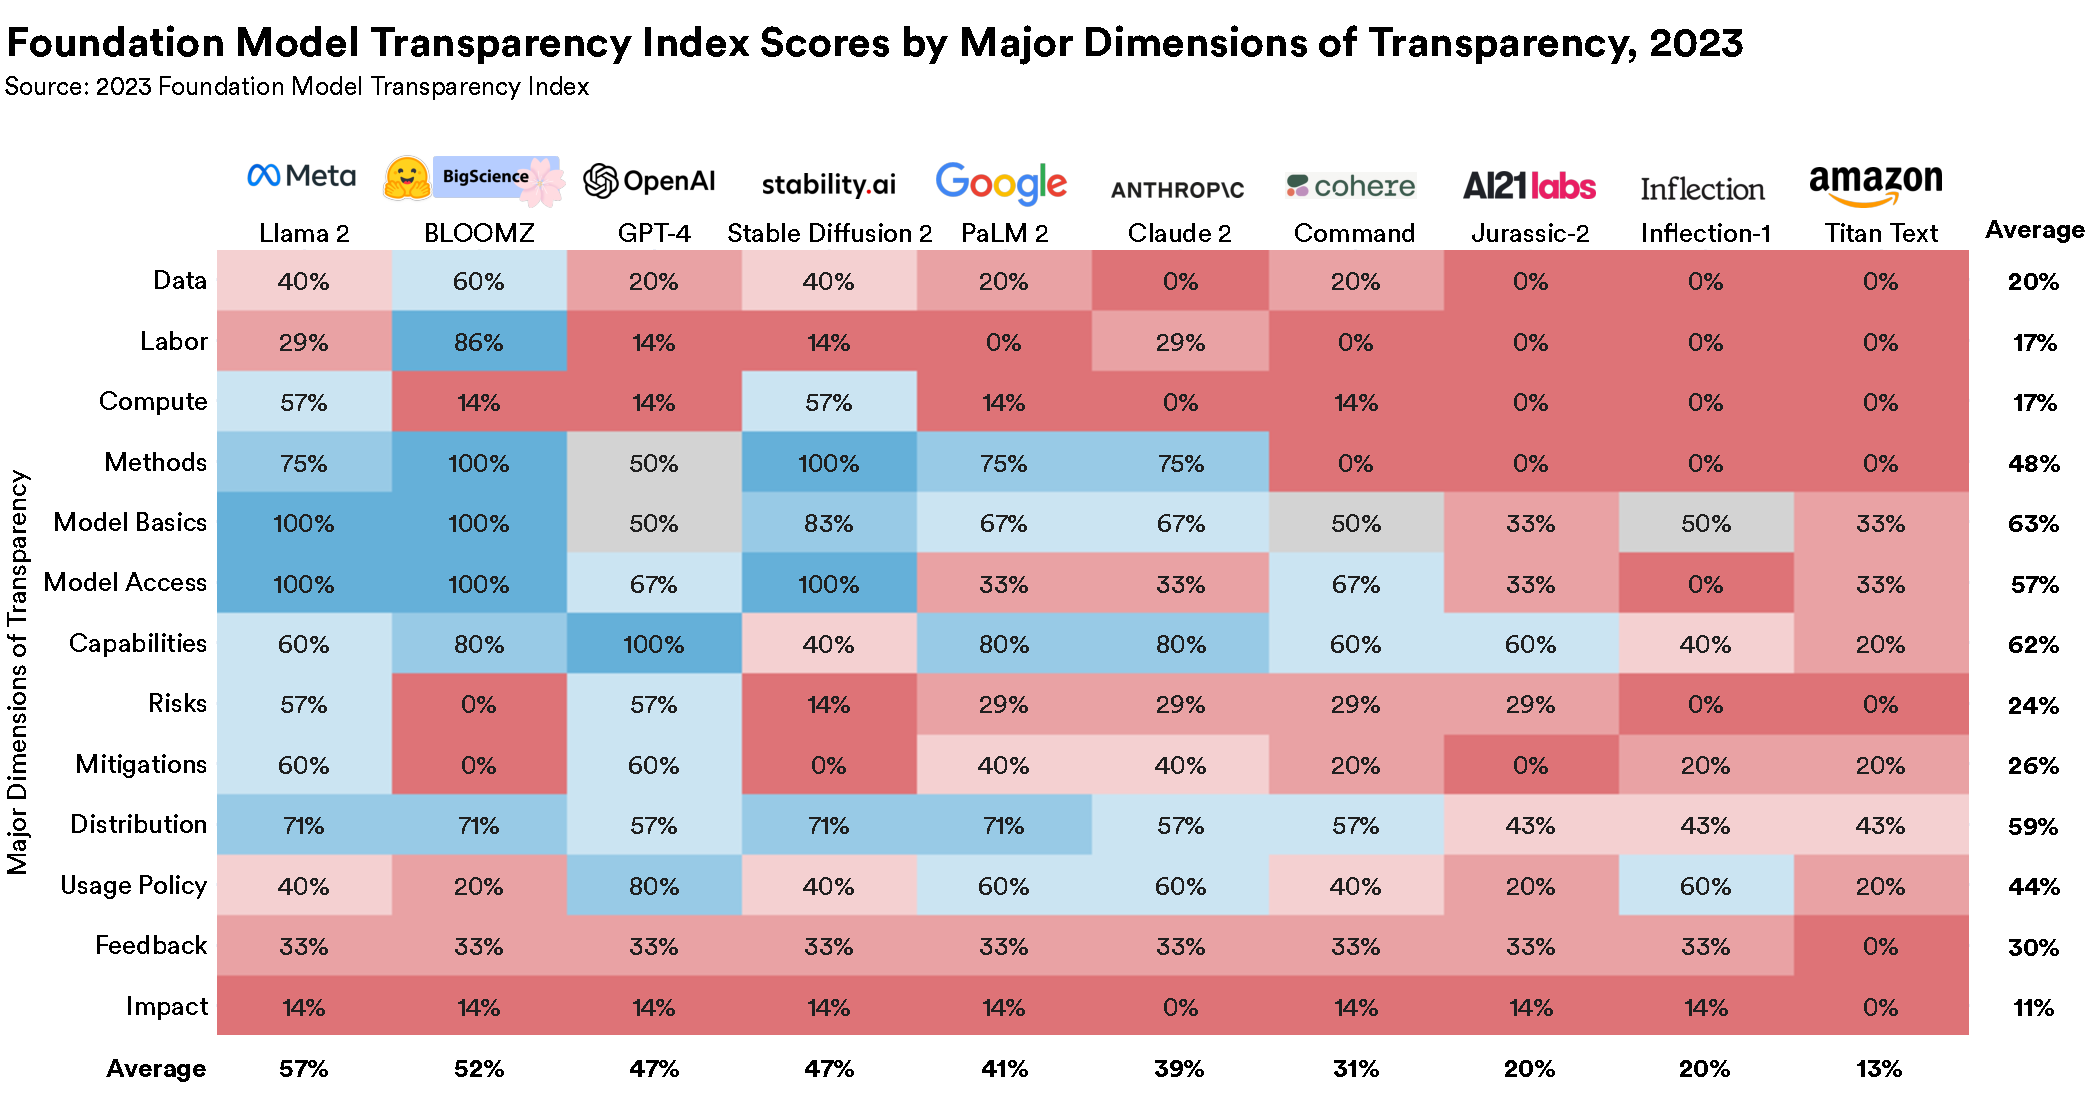
\includegraphics[keepaspectratio, width=\textwidth]{figures/overall_scores.pdf}
\caption*{\textbf{Scores for \numcompanies major foundation model developers across \nummajorsubdomains major dimensions of transparency.}
}
\label{fig:major-subdomain-scores}
\end{figure*}
